\documentclass[10pt,a4paper]{article}

\usepackage[margin=0.65in]{geometry}
\usepackage{amsmath,booktabs,array}
\usepackage{graphicx}
\usepackage{fancyhdr}
\usepackage[hidelinks]{hyperref}

\graphicspath{{figures/}}
\setlength{\parindent}{0pt}
\setlength{\parskip}{0.4em}
\renewcommand{\arraystretch}{1.08}
\raggedbottom

\pagestyle{fancy}
\setlength{\headheight}{13pt}
\fancyhf{}
\lhead{Deep Learning Laboratory}
\rhead{Lab Assignment 6}
\cfoot{\thepage}

\newcommand{\captionexample}[5]{%
    \begin{minipage}[c][44mm][c]{\textwidth}
        \begin{minipage}[c]{0.26\textwidth}
            \centering\includegraphics[width=\linewidth,height=38mm,keepaspectratio]{#1}
        \end{minipage}\hfill
        \begin{minipage}[c]{0.71\textwidth}
            \small
            \textbf{#2}\par\vspace{1mm}
            \textbf{Reference 1:} #3\par
            \textbf{Reference 2:} #4\par
            \textbf{Generated:} #5
        \end{minipage}
    \end{minipage}\par
}

\begin{document}

\begin{center}
    {\Large\bfseries Deep Learning Laboratory -- Assignment 6}\par
    \vspace{1mm}
    {\small Team 17: Mirthula M (26120121), Karthikeyan M (26120004)}
\end{center}

\section*{1. Sentiment classification}

Fine-tuned GloVe 50d embeddings feed one vanilla tanh RNN with 64 hidden units.
Concatenated temporal mean/max pooling feeds a two-class classifier.
Training uses class-weighted cross-entropy and AdamW; validation macro F1 selects
checkpoint 9 from 17 epochs. The prediction threshold is fixed at 0.5.

Of 5,600 supplied training rows, 399 normalized-text test overlaps and
526 remaining duplicate text/label rows are removed before grouped validation.
Fit/validation/test sizes are $3740/935/1400$; labels and the supplied test split are unchanged.

\begin{center}
\small
\begin{tabular}{lrr}
\toprule
Score (\%) & Train (fit) & Test\\
\midrule
RNN accuracy & 95.13 & 93.57\\
Majority baseline (always Negative) & 93.13 & 92.50\\
RNN balanced accuracy & 80.99 & 72.02\\
\bottomrule
\end{tabular}
\end{center}

The test set has 1,295 Negative and 105 Positive labels: high accuracy alone is
misleading. Test positive recall is 46.67\%; duplicate test texts remain
(1,340 unique texts in 1,400 rows), so rows are not independent examples.

\section*{2. Image captioning}

Frozen ImageNet VGG16 features are globally averaged to 512 dimensions,
standardized using training statistics, and projected to a 64d context.
Each GloVe 50d word vector is concatenated with this context and passed to one
vanilla RNN (64 units), also initialized by the context. Embeddings are fine-tuned;
Adam minimizes token cross-entropy. Best validation loss selects epoch
22 of 28.

The seed-17 image-disjoint train/validation/test split is $3200/400/400$, with
five captions per image. Vocabulary and feature statistics use training data only.

\begin{center}
\small
\begin{tabular}{lrrrr}
\toprule
Split & BLEU-1 & BLEU-2 & BLEU-3 & BLEU-4\\
\midrule
Train & 0.6626 & 0.4970 & 0.3557 & 0.2477\\
Test & 0.5284 & 0.3494 & 0.2244 & 0.1425\\
\bottomrule
\end{tabular}
\end{center}

Scores are unsmoothed cumulative corpus BLEU (0--1), over the full train/test
splits with all five references. Evaluation is free-running beam search
(beam 3, length penalty $\alpha=0.7$, maximum sequence length 30), not teacher forcing.
The lower test BLEU indicates weaker caption generalization.

\begin{center}
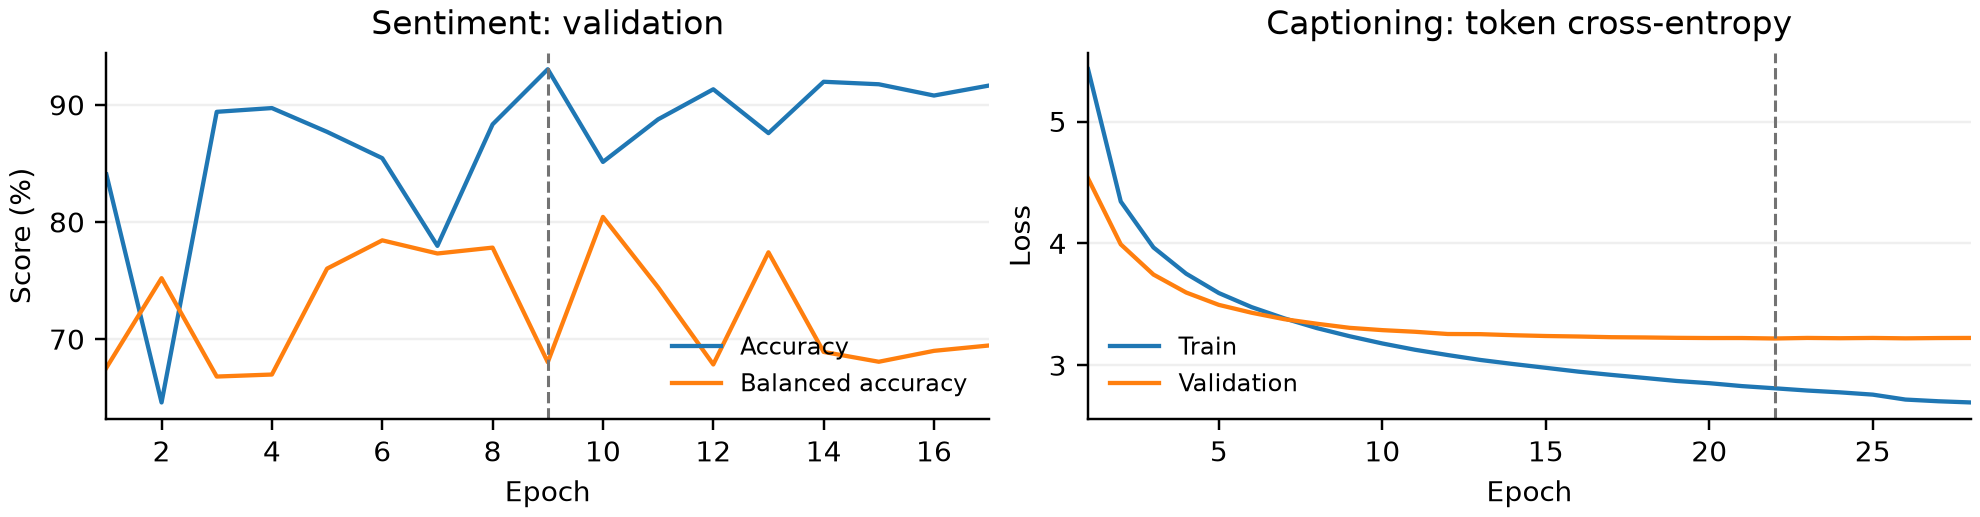
\includegraphics[width=\textwidth]{learning_curves.png}\par
{\footnotesize Dashed lines mark selected checkpoints.}
\end{center}

{\footnotesize Pretrained: Stanford GloVe 6B (50d); torchvision VGG16 ImageNet-1K V1.
The following galleries are random, not ranked; generated captions are unedited.}

\clearpage
\section*{3. Training image examples}

Five images sampled with seed 17 from sorted filenames; first two saved references shown.

\captionexample{train_1.jpg}
{1. 3413806271\_17b7e102aa.jpg}
{the people in the red parasail are gliding over the water}
{two people are hang gliding}
{two people are in the water}

\captionexample{train_2.jpg}
{2. 317641829\_ab2607a6c0.jpg}
{a man in a red coat stands outside of a store near a big column}
{a man in a red jacket and jeans stands next to a column in front of a store}
{a man in a red jacket is standing on a sidewalk}

\captionexample{train_3.jpg}
{3. 2865564810\_5c63328cd4.jpg}
{a biker doing a somersault with the bike in front of a crowd}
{biker performing jump while onlookers watch}
{a man is doing a trick on a ramp}

\captionexample{train_4.jpg}
{4. 3048461682\_e89f81b1c7.jpg}
{a dog runs over a stick in the leaves}
{a small white dog is jumping over a branch on the ground covered with leaves}
{a white dog is running through the grass}

\captionexample{train_5.jpg}
{5. 2822148499\_eaa46c99d4.jpg}
{a brown and white dog is looking at a tennis ball floating in a pool}
{a brown and white dog looking into a pool at a tennis ball}
{a white dog is jumping over a tennis ball}

\clearpage
\section*{4. Test image examples}

Five images sampled with seed 17 from sorted filenames; first two saved references shown.

\captionexample{test_1.jpg}
{1. 3350260112\_fcb47ff6b2.jpg}
{lots of people are playing in the river that runs through the city and in the sandy park beside it}
{lots of people play in the water at the beach}
{a group of people are in the water}

\captionexample{test_2.jpg}
{2. 3173014908\_b3e69594b6.jpg}
{a person skiing downhill in the snow}
{a skier puffs up a cloud of snow}
{a skier is going down a snowy hill}

\captionexample{test_3.jpg}
{3. 2842609837\_b3a0b383f7.jpg}
{a group of four friends are drinking alcohol at a party}
{a man wearing black stands with three woman who have blonde hair}
{two men are posing for a picture}

\captionexample{test_4.jpg}
{4. 3041487045\_b48ac7ed08.jpg}
{a dog runs through the woods}
{a pale tan dog romps through a wooded area}
{a dog runs through the snow}

\captionexample{test_5.jpg}
{5. 2782480767\_064c95eff2.jpg}
{a girl holds her breath underwater in a pool}
{a girl is about to emerge from a swimming pool}
{a little girl in a blue shirt is sliding down a water slide}

\end{document}
